\chapter{GNU Radio}

\section{Introduction}
GNU Radio is a free \& open-source software development toolkit that provides signal processing blocks to implement software radios. It can be used with readily-available low-cost external RF hardware to create software-defined radios, or without hardware in a simulation-like environment. It is widely used in hobbyist, academic and commercial environments to support both wireless communications research and real-world radio systems.

\section{What does GNU Radio do?}
It does all the signal processing. You can use it to write applications to receive data out of digital streams or to push data into digital streams, which is then transmitted using hardware.

GNU Radio has software equivalents of real world radio system components like filters, demodulators, equalizers, etc. These are usually referred to as blocks. You can create a complex system by connecting various blocks. If you cannot find some specific blocks, you can even create your own blocks and add them.

Most of GNU Radio has been implemented using the Python programming language, and the performance-critical parts have been implemented using C++. Typically, a GNU Radio user writes his applications in Python, unless he has some performance-critical needs. Thus, GNU Radio gives its users an easy-to-use, rapid application development environment.

\section{GNU Radio with USRP}

\begin{figure}[h]
\centering
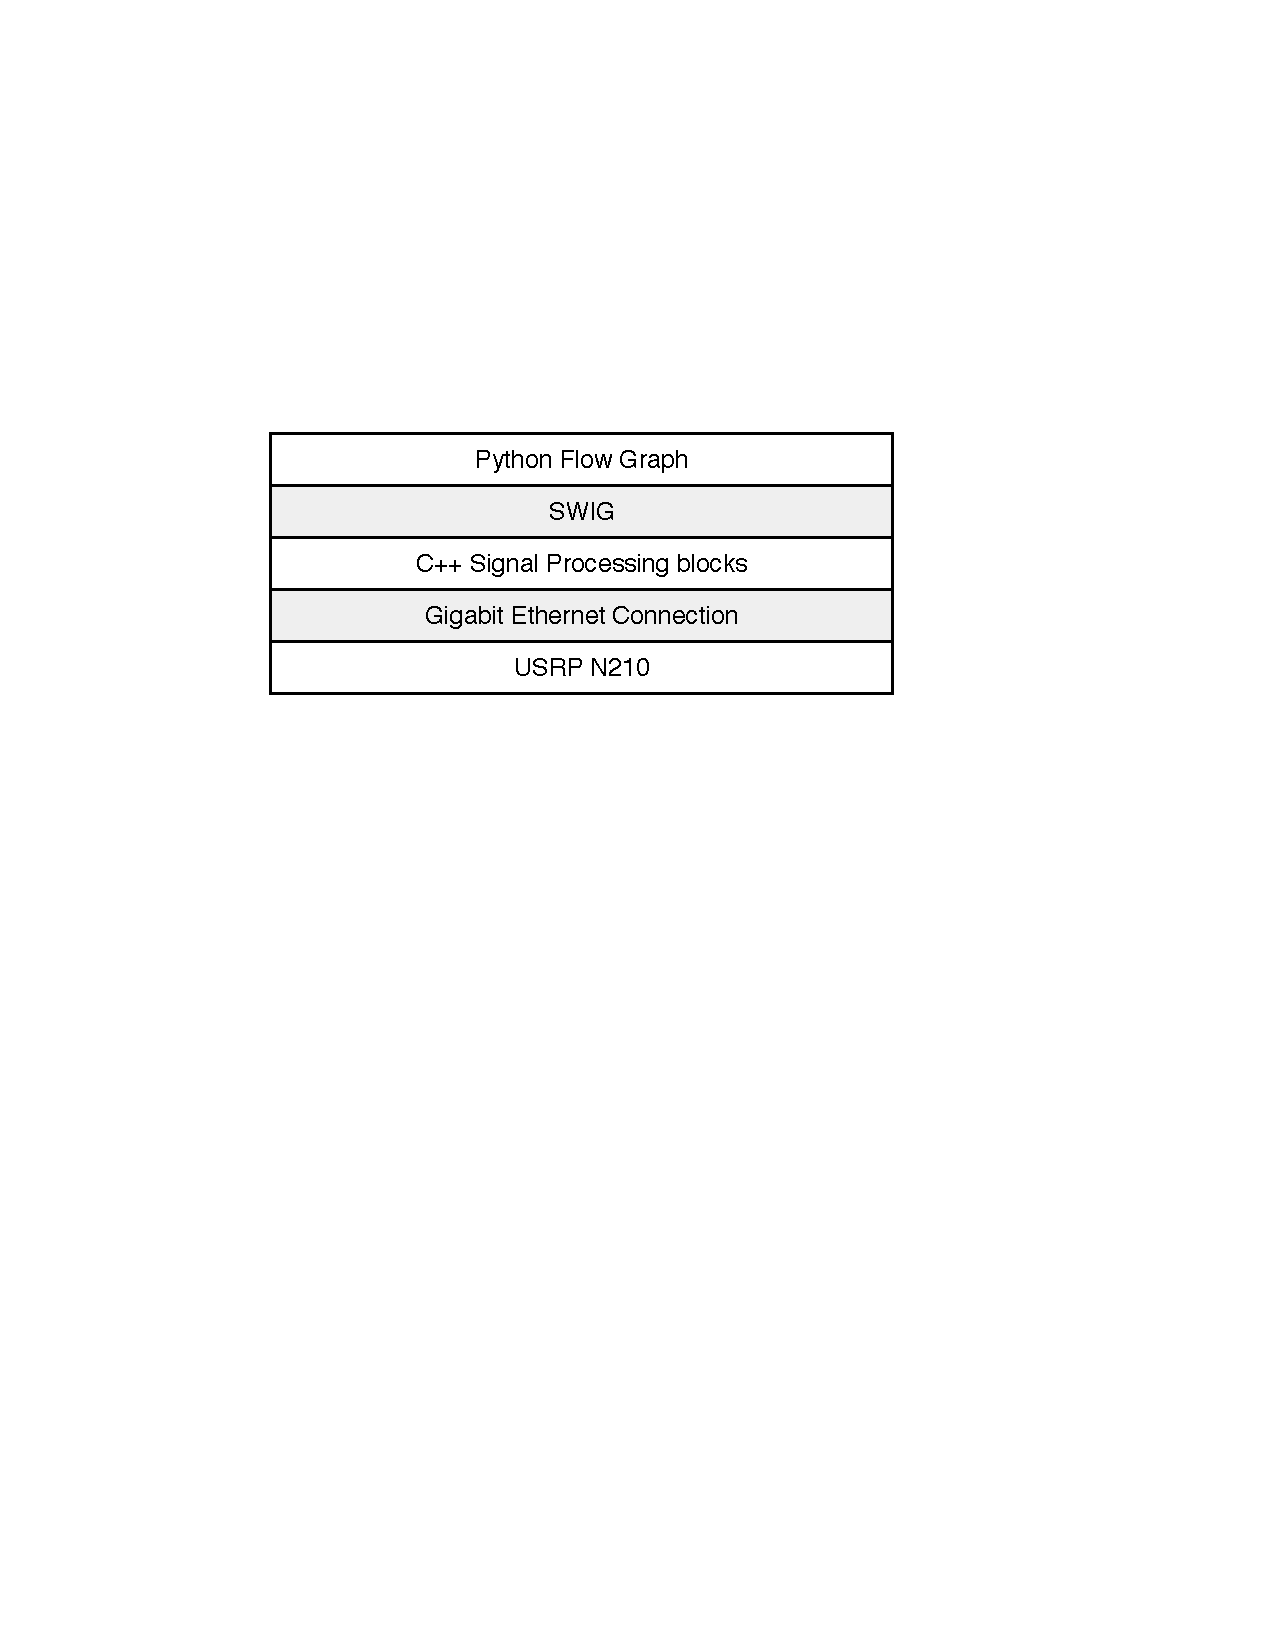
\includegraphics[width=1\textwidth]{gnuradio_architecture}
\caption{Architecture of GNU Radio}
\label{gnuradio_architecture}
\end{figure}

The USRP and the host computer make up the hardware part of the SDR system. The host computer must run a compatible software package such as GNU Radio or Simulink to complete the SDR system. In this project we are using GNU Radio as the software platform.

GNU Radio communicates with the USRP through the USRP Hardware Driver (UHD) software. The UHD provides a host driver and an Application Programming Interface (API) for the USRP. GNU Radio uses the UHD to set user-specified parameters like RF center frequency, antenna selection, gain, sampling rate, interpolation, decimation, etc.
